\documentclass{scrartcl}
\usepackage[utf8]{inputenc}
\usepackage{amsmath, amsfonts,amssymb}
\usepackage{graphicx}
\usepackage{xcolor}
\usepackage{caption}
% \usepackage{algorithmicx}
% \usepackage{algorithm}
% \usepackage[noend]{algpseudocode}
% \usepackage{booktabs}
% \usepackage{mathtools}
% \usepackage{float}
% \usepackage{floatpag}
% \usepackage{comment}
% \usepackage{cases}
% \usepackage{mathtools}

%%%%%% PREAMBLE

\newtheorem{theorem}{Theorem}
\newtheorem{lemma}{Lemma}
\DeclareMathOperator*{\argmax}{arg\,max}
\DeclareMathOperator*{\argmin}{arg\,min}
\DeclareMathOperator*{\unif}{Unif}
\DeclareMathOperator*{\bin}{Bin}

\newcommand{\todo}[1]{\textcolor{red}{TODO:
    #1}\PackageWarning{TODO:}{#1!}}

\newcommand{\N}{\mathbb{N}} % naturals
\newcommand{\Q}{\mathbb{Q}} % rationals
\newcommand{\Z}{\mathbb{Z}} % integers
\newcommand{\R}{\mathbb{R}} % reals
\newcommand{\ep}{\varepsilon}
\newcommand{\expect}[1]{\operatorname{\textnormal{\textbf{E}}}\left[#1\right]}
\newcommand{\prob}[1]{\operatorname{\textnormal{Pr}}\left(#1\right)}

\begin{document}

Since we don't have temporal (pre-intervention) data, autocorrelation
refers to spatial autocorrelation throughout.

\section{Global autocorrelation of infestation}
\label{sec:glob-autoc-infest}

Although used in a similar study \cite{Lucero2013}, using ArcGIS's AVG
NEAREST NEIGHBOR function is maybe not appropriate here, since one of
the assumptions of this method is that points are free to locate
anywhere in the study area. This is particularly untrue for infested
houses, since these can only appear where there are houses. A more
appropriate analog to identify whether infestations are clustered is a
permutation test.

Figure \ref{fig:perm-test} shows a simulated distribution obtained
from repeatedly shuffling the infestation status of houses within each
village, then measuring the mean distance between infested
houses. Based on this simple permutation test, only the villages
Prensa and Paternito show a global pattern of infestation. Indeed,
Amatillo shows marginal evidence of dispersal, with infested houses
being further apart than expected from a random configuration.

Previously, I calculated Moran's I as a summary of the village-wide
extent of autocorrelation, and found significant clustering in all
villages except Cerr\'on. Since this statistic measures a different
phenomenon, the interpretation of the two should be compared. Moran's
I measures autocorrelation (while in this case controlling for
distance with the weight matrix $W$), which means a significant I
value likely indicates non-random patterns of both infestation and
non-infestation. The permutation test measures distance between
infested houses alone, which in addition to viewing neighborhood
effects differently than a test for correlation, only reflects
patterns of infestation. Also, the permutation test is not sensitive
to a choice of $W$.

\begin{figure}
  \centering
  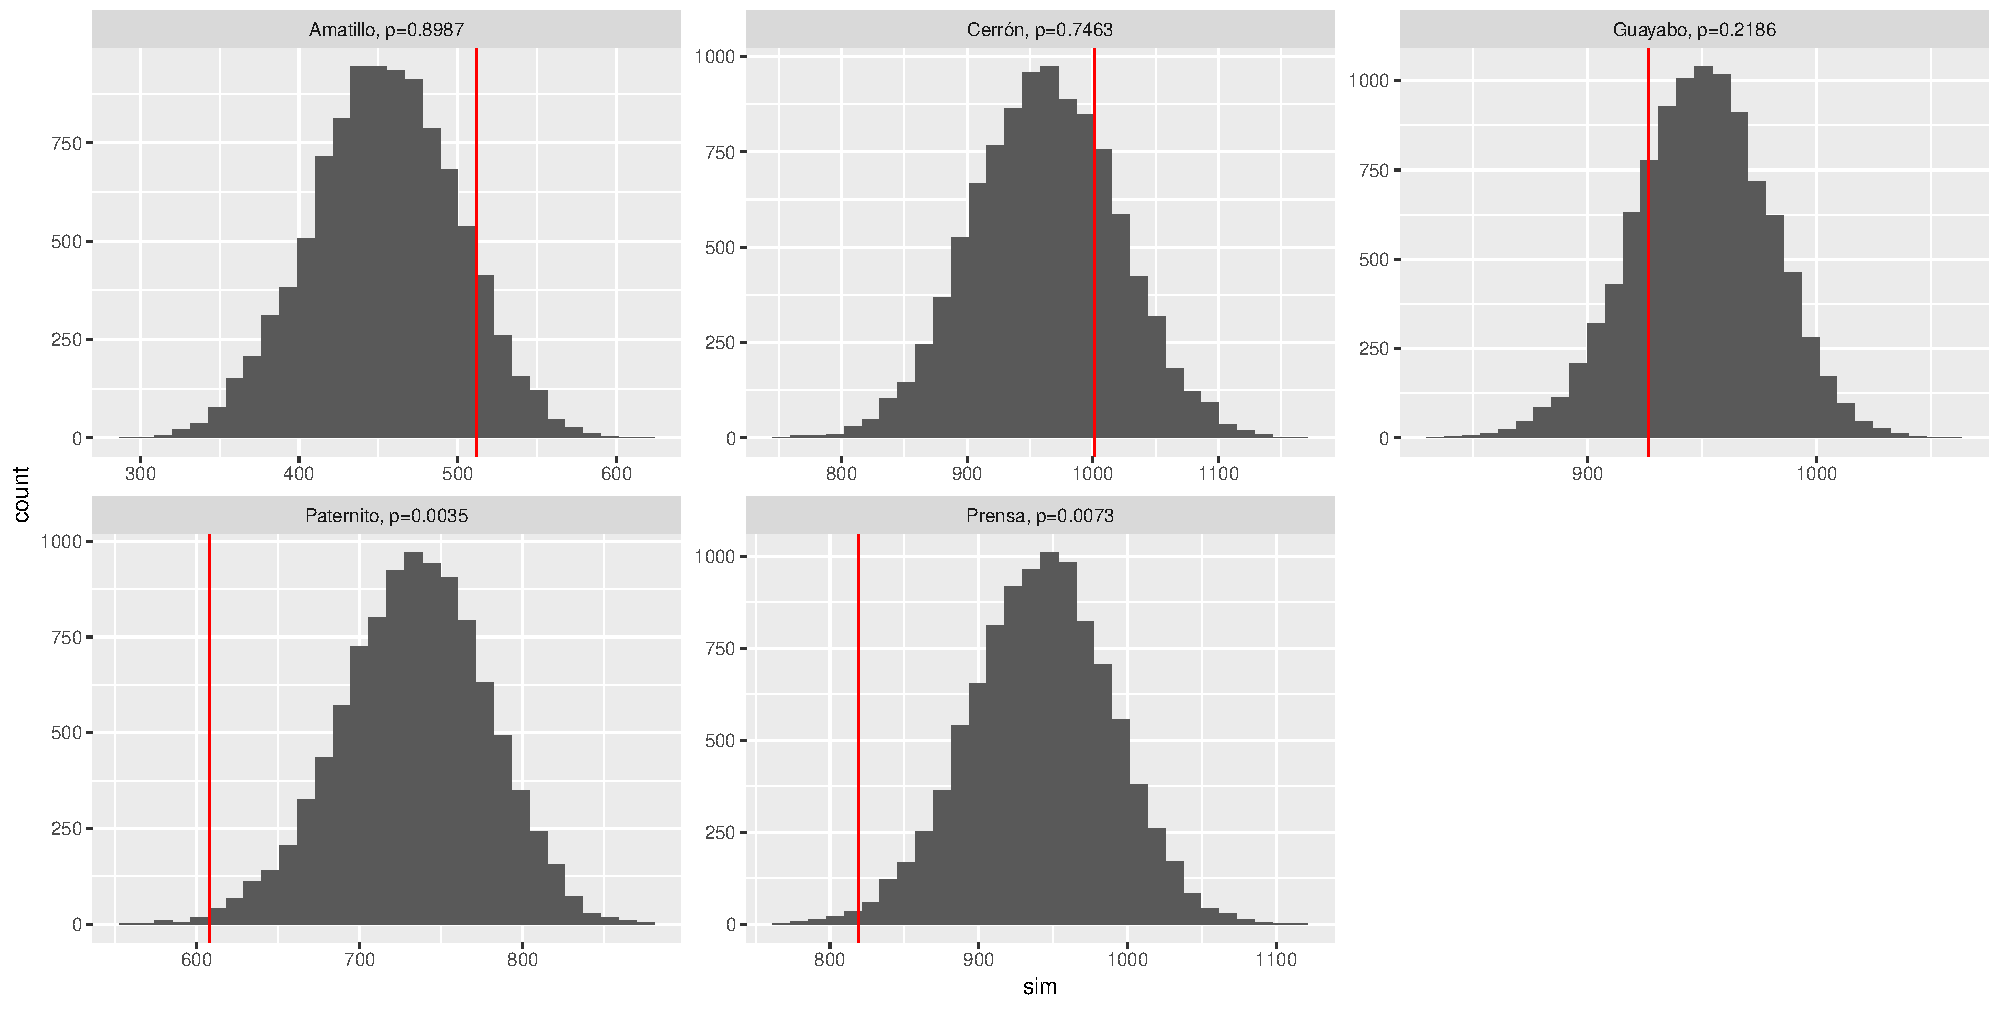
\includegraphics[width=.7\linewidth]{perm-test}
  \caption{Simulated distribution of mean distance between infested
    houses in each village. Each distribution obtained from 10,000
    draws. Red line indicates observed mean distance between infested
    houses. P-value obtained from one-sided hypothesis test that
    observed distance is less than theoretical distribution, i.e. the
    proportion of samples with mean distance less than observed.}
  \label{fig:perm-test}
\end{figure}

Another popular hypothesis is that houses closer to the village
periphery, in particular, to surrounding forested areas are more
likely to be infested. However, in the case of these villages, houses
generally appear interspersed within a matrix of forest, brush, and
farmland (Figures \ref{fig:prensa-earth-2011} and
\ref{fig:guayabo-earth-2020}). Therefore, any well-defined
specification of distance from forested areas would likely be
difficult. That said, it is possible that forested areas outside of
the circumference are more intact and less disturbed, and that this
would increase the exposure of sylvatic infestation for houses closer
the periphery.

To test whether houses near the surrounding forest saw infestation
than expected, we again use a permutation test by shuffling the
infestation status of houses and calculating the mean distance of the
simulated infestation labels from the edge of the village, defined
here as 50m from the convex hull of all houses in the village. We then
compared this simulated distribution to the observed mean distance; in
all villages, there was not particularly significant evidence that
infested houses tended to be closer to the periphery, though the
strength of this signal varied by village (see Figure
\ref{fig:perimeter-test}).

\begin{figure}
  \centering
  \includegraphics[width=.7\linewidth]{google-earth/prensa-earth-2011}
  \caption{Village of Prensa, Guatemala. Image from Google Earth
    taken in 2011, with georeferenced houses as added layer. Infested
    houses are red, while uninfested houses are white.}
  \label{fig:prensa-earth-2011}
\end{figure}

\begin{figure}
  \centering
  \includegraphics[width=.7\linewidth]{google-earth/guayabo-earth-2020}
  \caption{Village of Guayabo. Image from Google Earth
    taken in 2020 due to presence of cloud cover in 2011.}
  \label{fig:guayabo-earth-2020}
\end{figure}

\begin{figure}
  \centering
  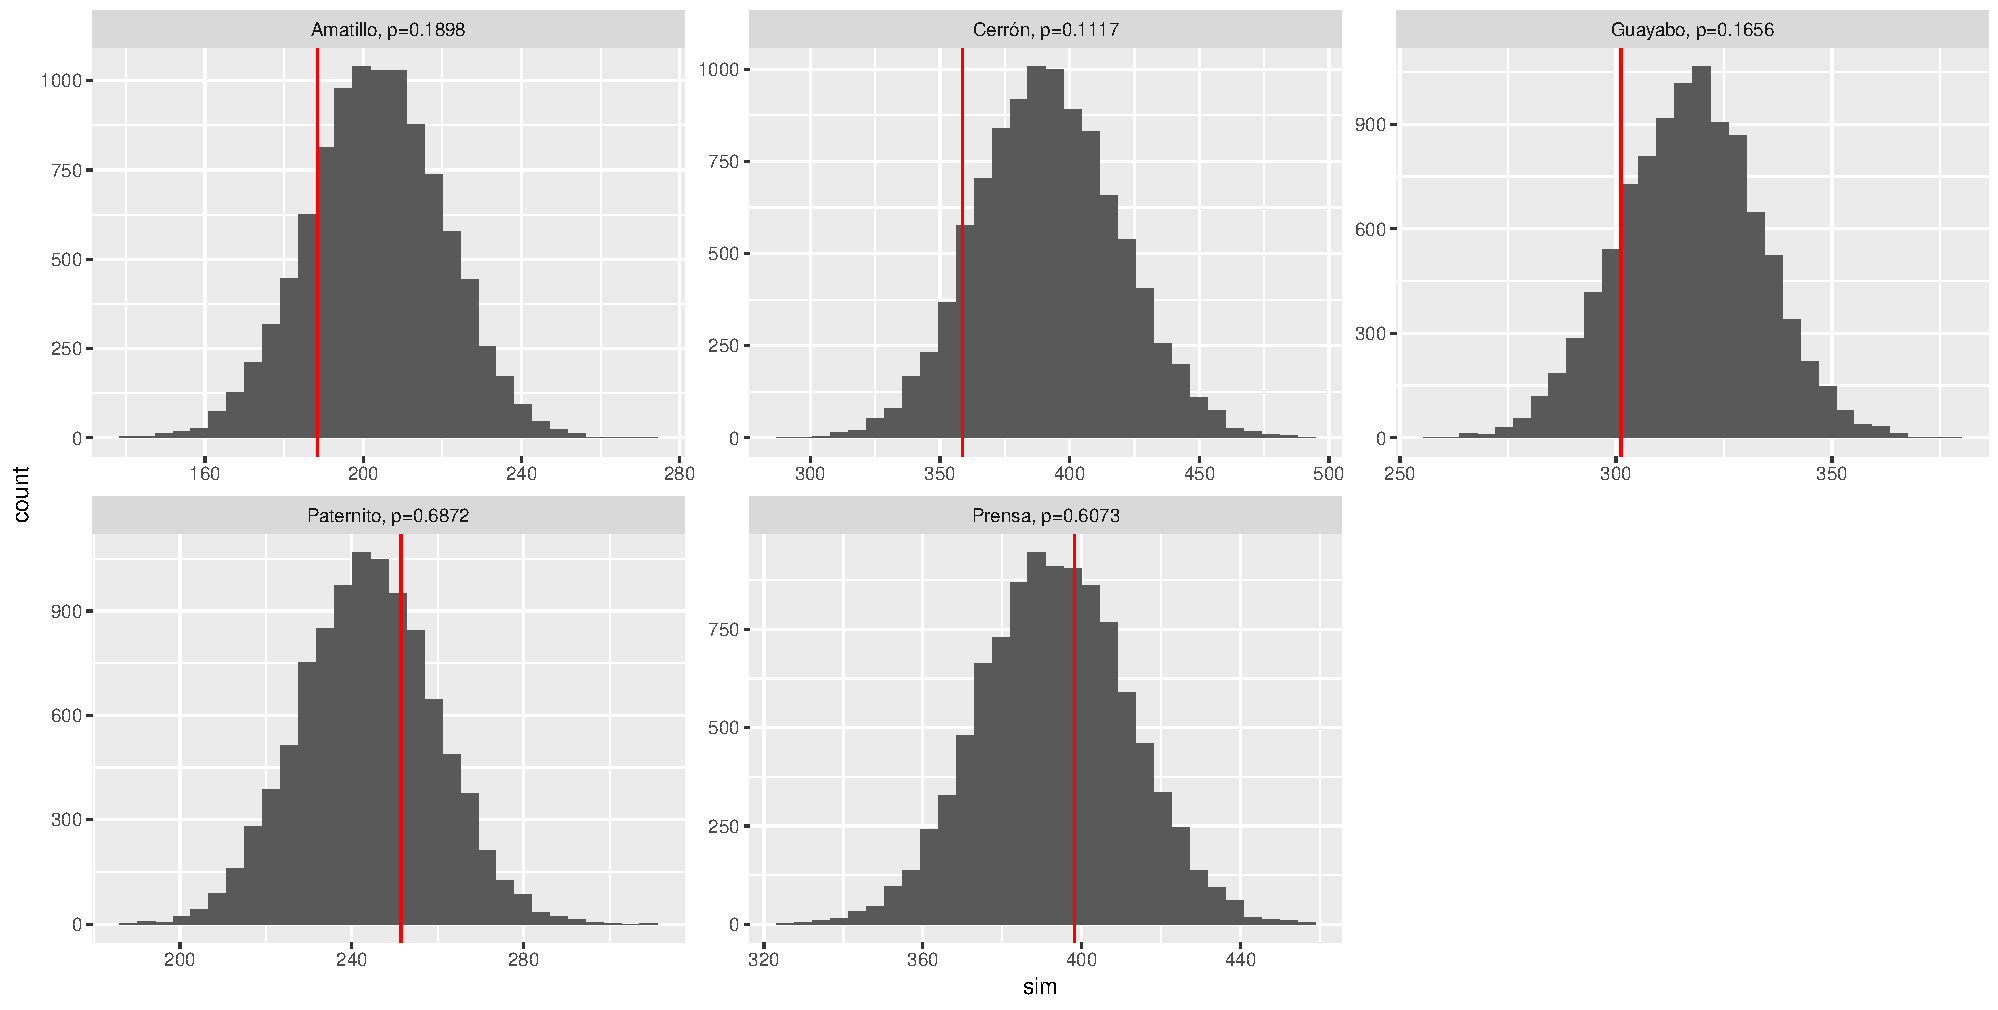
\includegraphics[width=.7\linewidth]{perimeter-test}
  \caption{Results from permutation test (draws=10,000) of expected
    mean distance of infested houses from village periphery, compared
    to the observed mean distance. Several villages show very mild
    evidence that the observed distance of infested houses from
    village edge is non-random.}
  \label{fig:perimeter-test}
\end{figure}

\section{Local autocorrelation of infestation}
\label{sec:local-autoc-infest}

We now turn to examining the so-called ``local autocorrelation'' of
infestation. In contrast to global statistics which summarize the
extent of correlation throughout the entire village, local statistics
look for spatial clustering within particular neighborhoods, hence
summarizing the extent of autocorrelation for each observation. One recent measure of local autocorrelation well suited for data with a mix of binary, ordinal, and continuous variables is the ELSA statistic \cite{Naimi2019}. However, one limitation is this measure depends on defining a neighborhood size, and it is not clear which radius is best for this application. One way we can infer good choices is by examining the average ELSA statistic as a function of distance using a so-called ``entrogram'' (Figure \ref{fig:entrogram}). Figure \ref{fig:elsa-amatillo} shows the ELSA scores at several neighborhood sizes in Amatillo. It appears that the quick initial jump in Amatillo's entrogram is due to very few houses being within 30m of each other. The downward slope in spatial structure 100-400m is more interesting. One explanation for this unexpected trend is many infestations are concentrated in small pockets at the periphery. This causes the entropy of larger neighborhoods to go down, since all neighborhoods become dominated by the many uninfested houses towards the village center, so this component of the ELSA statistic is low and similar across the whole village. Examine individual components of the ELSA statistic could confirm this.

Finally, we compare the entrogram results to a semi-variogram (Figure \ref{fig:semivar}). Several villages show a rapid breakdown of spatial structure, with the first few points being followed by a jump in semi-variance followed by a relatively even cloud, while others show more clear patterns of autocorrelation and several scales, suggesting that in some villages it may be more important to use analyses with several choices of neighborhood radius. \todo{discuss reasons for differences and implications for Bayesian analysis}

\begin{figure}
  \centering
  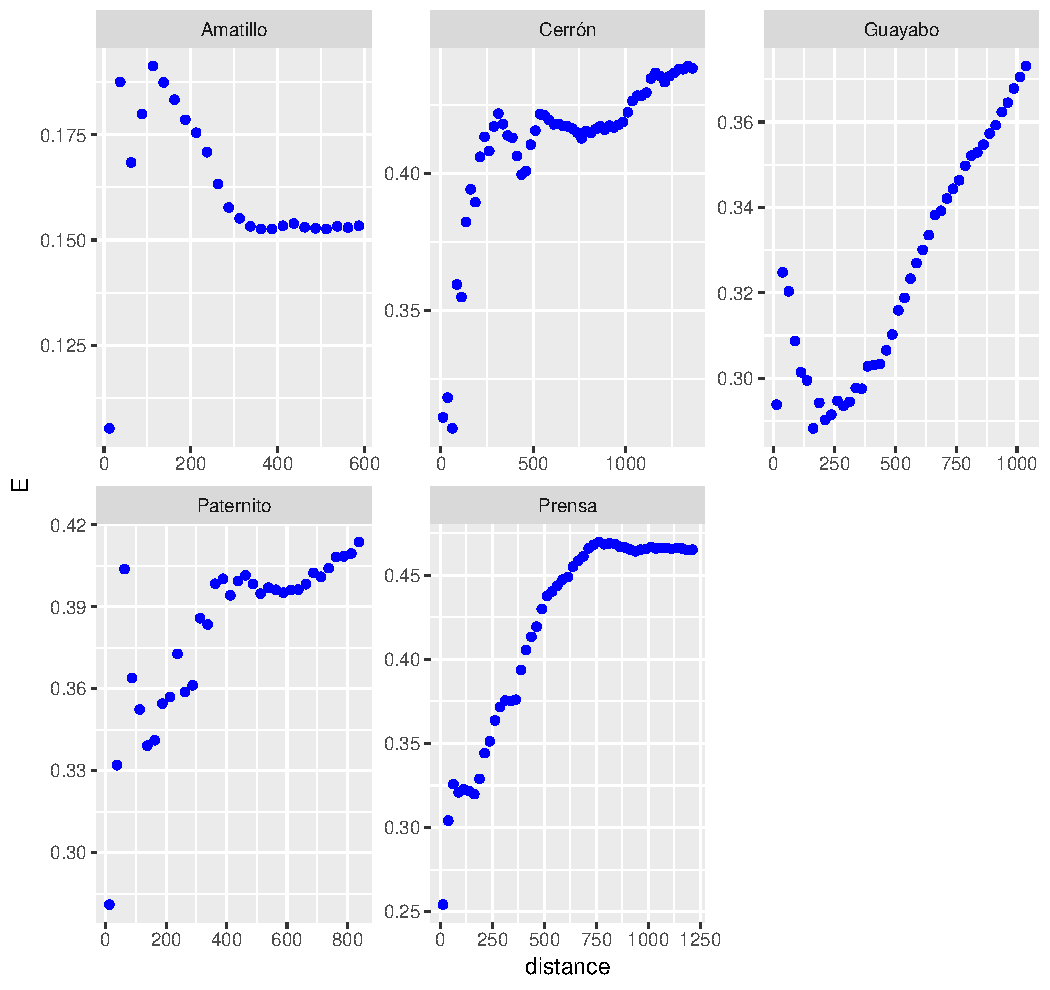
\includegraphics[width=.7\linewidth]{entrogram}
  \caption{Entrogram of infestation in each village, with a lag size
    of 25m up to a maximum of 1/2 times maximum distance between
    houses.}
  \label{fig:entrogram}
\end{figure}

\begin{figure}
  \centering
  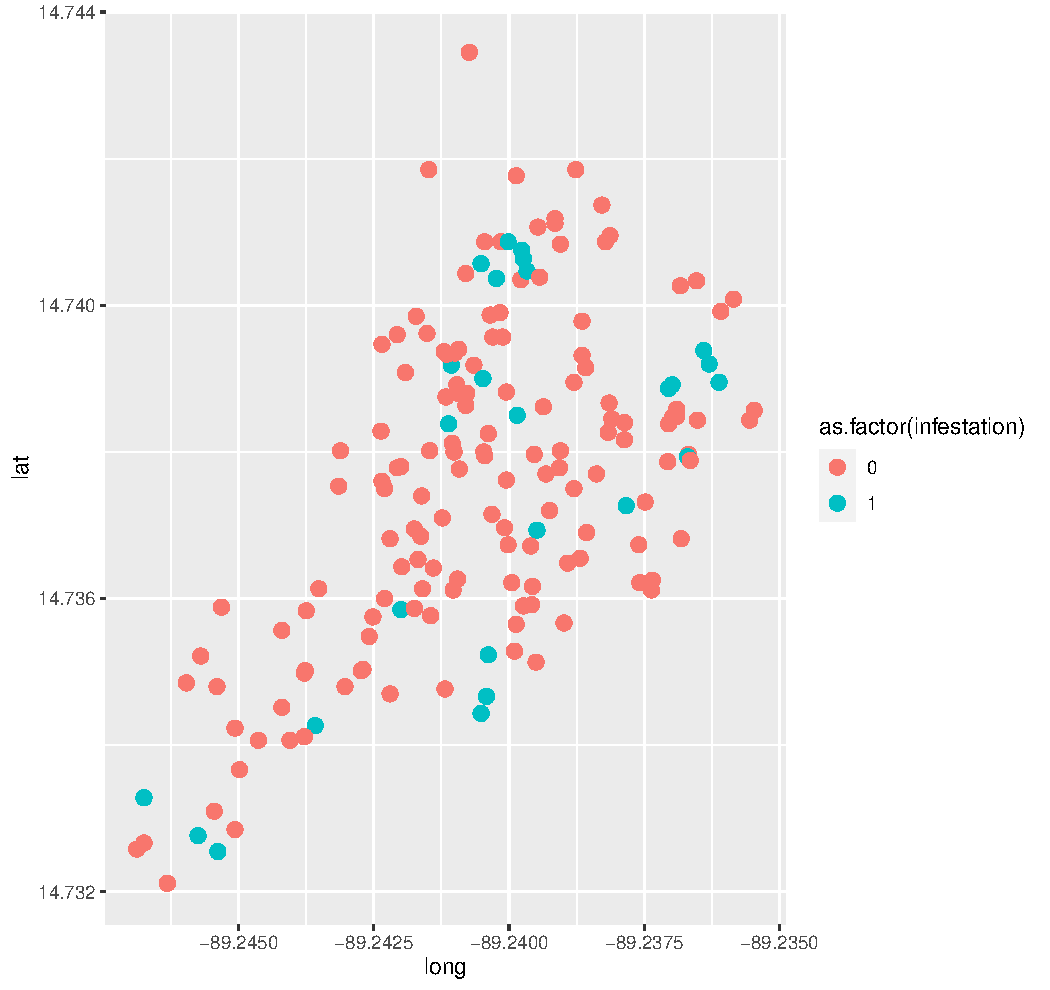
\includegraphics[width=.49\linewidth]{amatillo-inf-dist}
  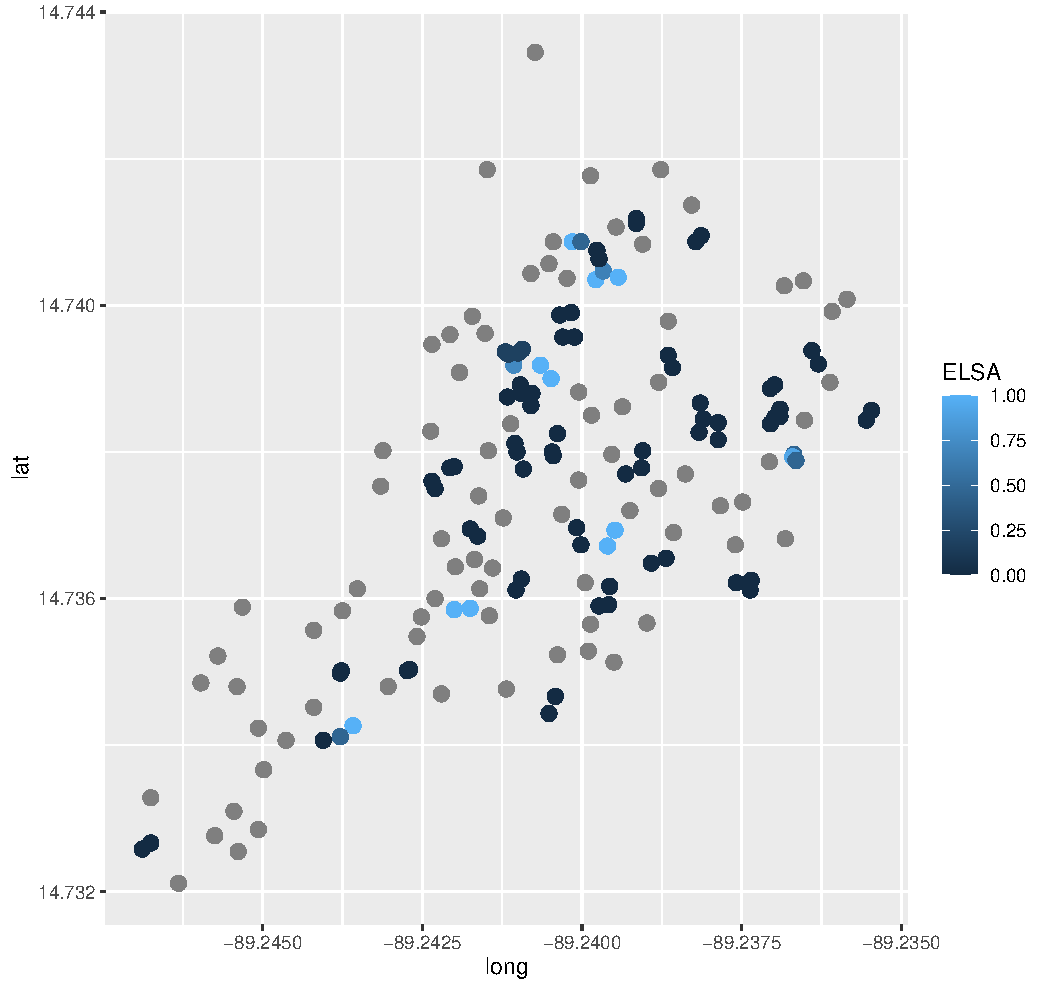
\includegraphics[width=.49\linewidth]{elsa-amatillo-30}
  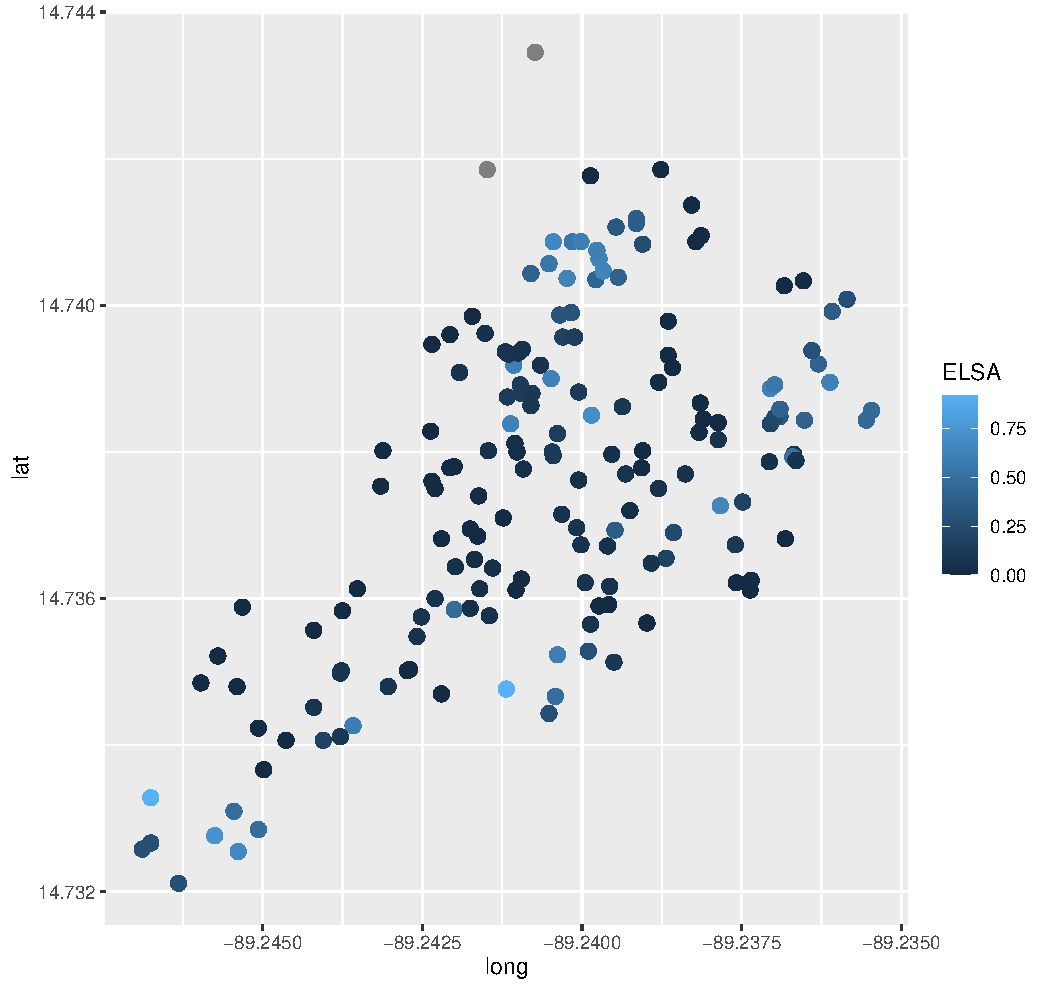
\includegraphics[width=.49\linewidth]{elsa-amatillo-100}
  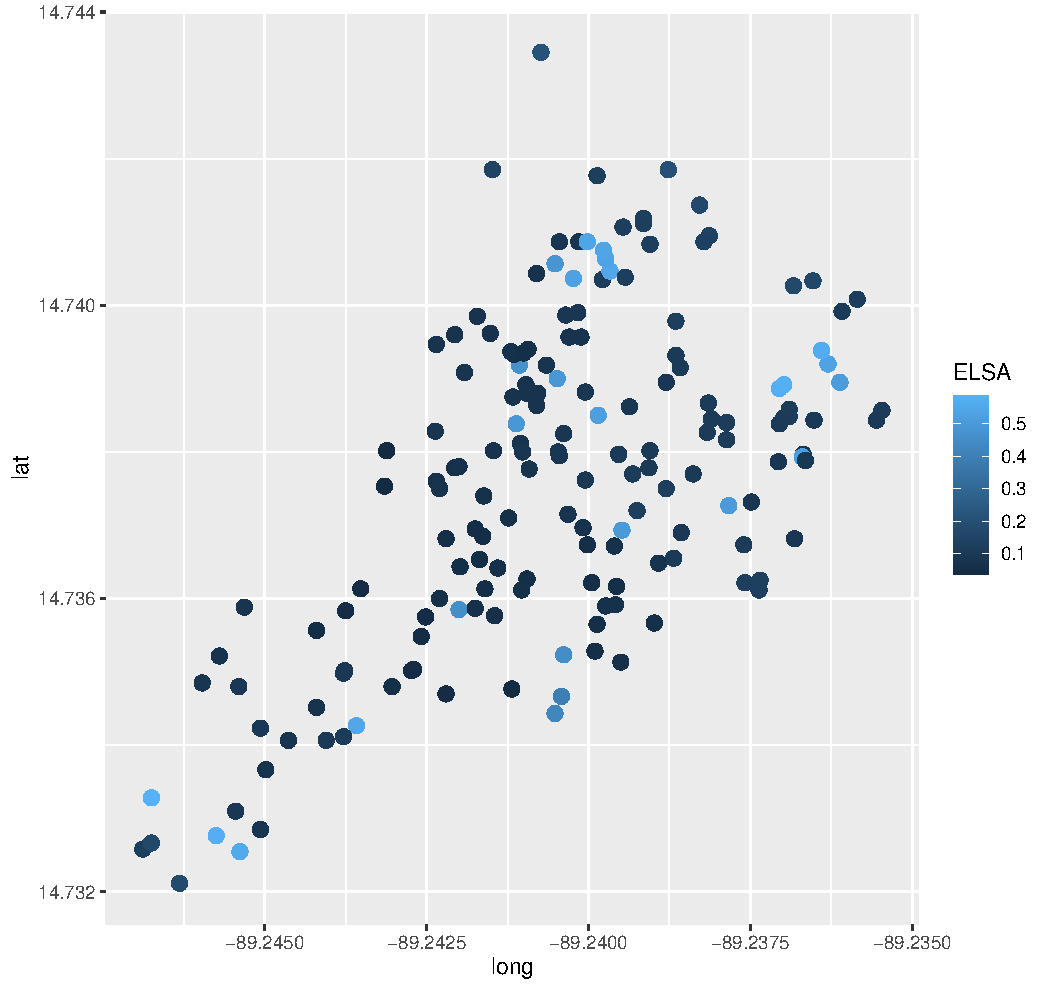
\includegraphics[width=.49\linewidth]{elsa-amatillo-400}
  \caption{Reading from left to right: distribution of infestation in
    Amatillo for reference, then the local ELSA score with radii 30,
    100, and 400m. Gray indicates house had no neighbor with radius.}
  \label{fig:elsa-amatillo}
\end{figure}

\begin{figure}
  \centering
  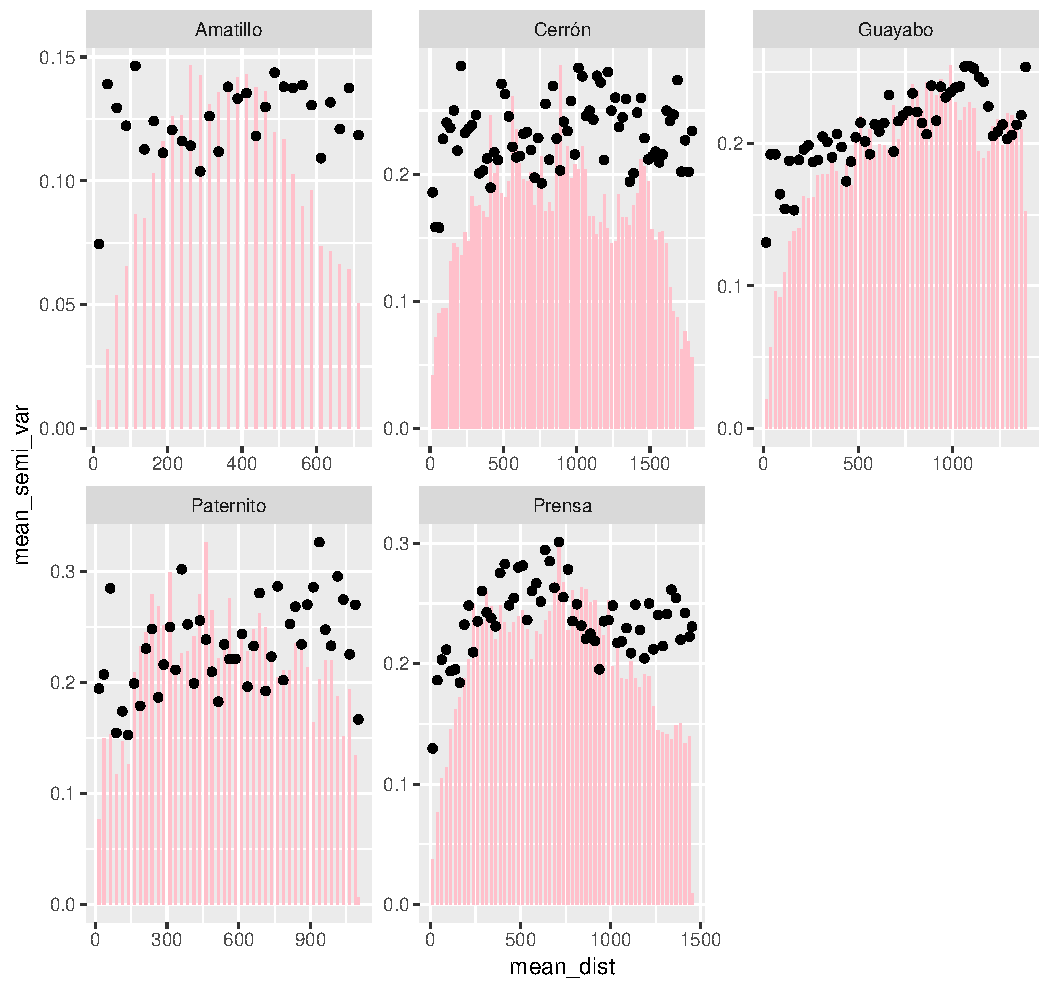
\includegraphics[width=.7\linewidth]{semivar}
  \caption{Indicator variogram of infestation with lag size of 25m and
    max distance of 1/2 maximum distance between houses. Pink bars indicate relative size (number of pairs) of each bin.}
  \label{fig:semivar}
\end{figure}

\section{Cross-variance of infestation with socio-economic factors}
\label{sec:cross-vari-infest}

\todo{Include plot with PC1, but also revisit something that preserves the actual covariates}

\section{Takeaways for Bayesian analysis}
\label{sec:take-bayes-analys}

\begin{itemize}
\item Amatillo infestations is the spatial oddball of the group. This
  means it maybe isn't a good initial testing ground, but good to come
  back to to compare to other villages.
\end{itemize}

\bibliographystyle{alpha}
\bibliography{C:/Users/brendandaisy/Documents/citations/chagas}

\end{document}
%%% Local Variables:
%%% mode: latex
%%% TeX-master: t
%%% End:
